\chapter{Introduction}
This document will include the BAT (Bolt Analysis Tool) User Manual \cite{ESAPSS} \cite{ECSS_HB_32_23A} \cite{VDI2230_1}.

\chapter{Bolt and Thread Geometry}
$D_{Km}$ is the \emph{effective diameter of under head/nut friction torque} and is defined by 
\begin{equation}
  D_{Km} = \frac{D_{hole}+d_h}{2}
  \label{equ:dkm}
\end{equation}
where $D_{hole}$ is the \emph{through-hole diameter} in the clamped parts and $d_h$ is the 
\emph{minimum bearing surface outer diamter} of the bolt head or nut. An other input value to calculate
the under-head friction torque \equ{equ:Muh} is the \emph{under head bearing angle} $\lambda$ seen in 
\fig{fig:ecss_uh_brg_angle}.
\begin{figure}[!htpb]
  \centering
  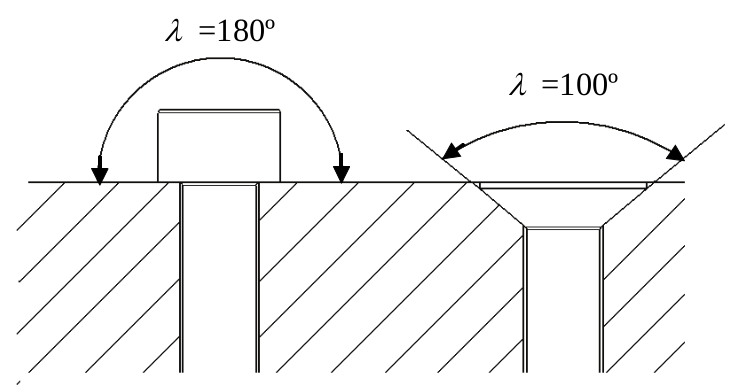
\includegraphics[width=0.5\textwidth]{ECSS_uh_brg_angle.png}
  \caption{Definition of under head bearing angle \cite{ECSS_HB_32_23A}}
  \label{fig:ecss_uh_brg_angle}
\end{figure}

\chapter{Joint Diagram}
\label{ch:jointdiag}
The \emph{joint diagram} seen in \fig{fig:joint_diagram} \cite{VDI2230_1} visualizes the forces and 
displacements and helps to understand the loading conditions of a concentrically loaded bolted joint. 
\begin{figure}[!htpb]
  \centering
  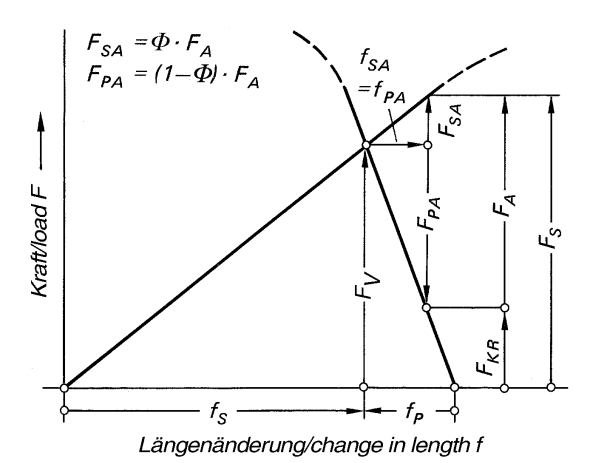
\includegraphics[width=0.7\textwidth]{VDI2230_Bild24.png}
  \caption{Joint diagram for the working state of a concentrically loaded \\ bolted joint with $n=1$ \cite{VDI2230_1}}
  \label{fig:joint_diagram}
\end{figure}

The preload force $F_V$ (see §\ref{sec:preload}) compresses the clamped parts $f_P$ and elongates
the bolt $f_S$ during tightening. If an external load $F_A$ is acting on the bolted joint the bolt
is streched much further and the clamped parts are relaxed ($f_{SA}=f_{PA}$) due to the loading. 
The \emph{additional axial bolt load} $F_{SA}$ and the \emph{additional axial plate load}\footnotemark[1]
\footnotetext[1]{If the bolt is loaded in tension $F_{PA}$ is better described as an 
\emph{axial plate relaxation force}.} $F_{PA}$ are given to
\begin{equation}
  F_{SA} = n \Phi F_A, \qquad F_{PA} = (1-n \Phi) F_A
  \label{equ:FSA_FPA}
\end{equation}
where $\Phi$ is the load factor, which is defined as the quotient of the additional bolt load $F_{SA}$ 
and the axial working load component $F_A$. $n$ is the \emph{load introduction factor} and is crucial
for determining the size of the additional botl loads. As seen in \fig{fig:joint_diagram} $F_{KR}$ is the residual
clamping load at the interface during relief or loading by $F_{PA}$ and after embedding in service and 
$F_S$ is the maximum bolt load. 

\chapter{Method B: ECSS-E-HB-32-23A}
This chapter provides a quick overview and summary of the equations used in \bat. A detailed description
can be found in the complete ECSS-E-HB-32-23A ESA handbook \cite{ECSS_HB_32_23A}. Some used variables
in the following equations have been changed compared to \cite{ECSS_HB_32_23A} by the author to increase
clarity and consistency.

\section{Preload and Torques}
\label{sec:preload}
The torque present at the thread interface $M_{th}$ is dependent of the \emph{axial bolt preload} $F_V$ 
and is given by
\begin{equation}
  M_{th} = F_V \tan(\varphi+\rho)\frac{d_2}{2}
\end{equation}
and the \emph{under-head torque} $M_{uh}$ due to friction between bolt head or nut and the adjacent 
clamped part (or shim) is defined by
\begin{equation}
  M_{uh} = F_V \frac{\mu_{uh} D_{Km}}{2} \frac{1}{\sin{\nicefrac{\lambda}{2}}}
  \label{equ:Muh}
\end{equation}
where $\lambda$ is the \emph{under head bearing angle} seen in \fig{fig:ecss_uh_brg_angle}.
It is assumed that the friction force for $M_{uh}$ is acting at mean bearing radius of the bolt head 
$D_{Km}$ \equ{equ:dkm}. $\varphi$ is the helix angle of the thread and $\rho$ is given by the relation
\begin{equation}
  \tan\rho = \frac{\mu_{th}}{\cos\nicefrac{\theta}{2}}
\end{equation}
where $\theta$ is the half angle of the thread groves (for Unified or Metric threads $\theta=60^\circ$).

The \emph{total installation torque} $T_A$ (without torque device scatter) applied to bolt head or nut
during tightening to produce the axial bolt preload $F_V$ is 
\begin{equation}
  T_A = M_{th} + M_{uh} + M_p
  \label{equ:TA}
\end{equation}
where $M_p$ is the \emph{prevailing torque} of the locking device. 
With the approximation $\tan\varphi \tan\rho \ll 1$ the expression $\tan(\varphi+\rho)$ can be written
as $\tan(\varphi+\rho) \approx \tan\varphi + \tan\rho$. Now equation \equ{equ:TA} can be rewritten to
\begin{equation}
  T_A = F_V \underbrace{ \left[ \frac{d_2}{2} \left( \tan\varphi + \frac{\mu_{th}}{\cos\nicefrac{\theta}{2}} \right) 
  + \frac{\mu_{uh} D_{Km}}{2 \sin\nicefrac{\lambda}{2}} \right]}_{K} + M_p
  \label{equ:TA2}
\end{equation}
where $K$ is the \emph{joint coefficient}.

For calculation of the minimum and maximum axial bolt preload, \bat implements the \emph{experimental coefficient method}
\cite{ECSS_HB_32_23A} with an explicit torque scatter torque of the tightening device $T_{scatter}$. Therefore
the minimum and maximum total installation torques are defined 
\begin{equation}
  T_A^{min} = T_A - T_{scatter} , \qquad T_A^{max} = T_A + T_{scatter}.
  \label{equ:Tscatter}
\end{equation}
To calculate the minimum and maximum \emph{axial bolt preload after tightening} $F_M^{min/max}$, 
\equ{equ:TA2} and \equ{equ:Tscatter} are combined 
\begin{equation}
  F_M^{min} = \frac{T_A^{min}-M_p^{max}}{K^{max}} ,\qquad
  F_M^{max} = \frac{T_A^{max}-M_p^{min}}{K^{min}}.
\end{equation}
If also the thermal influence and embedding is considered, this leads to the minimum and maximum
\emph{axial bolt preload at service} $F_V^{min/max}$
\begin{subequations}
  \setlength{\jot}{10pt}
  \begin{align}
    F_V^{min} &= \frac{T_A^{min}-M_p^{max}}{K^{max}}+\Delta F_{Vth}-F_Z \\
    F_V^{min} &= F_M^{min}+\Delta F_{Vth}-F_Z \\
    &= \frac{T_A^{min}-M_p^{max}}{\frac{d_2}{2} \left( \tan\varphi + \frac{\mu_{th}^{max}}
    {\cos\nicefrac{\theta}{2}} \right) + \frac{\mu_{uh}^{max} D_{Km}}
    {2 \sin\nicefrac{\lambda}{2}}}+\Delta F_{Vth}-F_Z
    \label{equ:FVmin}
  \end{align}
\end{subequations}
\begin{subequations}
  \setlength{\jot}{10pt}
  \begin{align}
    F_V^{max} &= \frac{T_A^{max}-M_p^{min}}{K^{min}}+\Delta F_{Vth} \\
    F_V^{max} &= F_M^{max}+\Delta F_{Vth} \\
    &= \frac{T_A^{max}-M_p^{min}}{\frac{d_2}{2} \left( \tan\varphi + \frac{\mu_{th}^{min}}
    {\cos \nicefrac{\theta}{2}} \right) + \frac{\mu_{uh}^{min} D_{Km}}
    {2 \sin \nicefrac{\lambda}{2}}}+\Delta F_{Vth}
    \label{equ:FVmax}
  \end{align}
\end{subequations}
where $\Delta F_{Vth}$ is thermal preload change (see §\ref{sec:thermal}) and 
$F_Z$ is the preload loss due to embedding (see §\ref{sec:embedding}).

\section{Thermal Influcence}
\label{sec:thermal}
If a thermal load is applied to a bolted joint, the bolt sees a change $\Delta F_{Vth}$ in the preload
force due to the CTE mismatch of bolt and clamped parts seen in \equ{equ:FVmin} and \equ{equ:FVmax}.
\subsection{Linear Thermal Influence}
For the following derivation it is assumed that the Young's Modulus $E$ of bolt and clamped parts does 
not change with temperature (temperature independent material properties). $c_b=\nicefrac{1}{\delta_b}$
and $c_c=\nicefrac{1}{\delta_c}$ are defined as bolt stiffness and clamp-part stiffness respectively.
Linear thermal elongation is defined
\begin{equation*}
  \varepsilon_{th} = \alpha \Delta T = \frac{\Delta l}{l_0}
\end{equation*}
The thermal elongation for bolt (index $b$) and clamped-parts (index $c$) are given to
\begin{subequations}
  \begin{align*}
    \Delta l_b &= \alpha_b \cdot \Delta T \cdot l_{0b} \\
    \Delta l_c &= \sum_i \alpha_{ci} \cdot \Delta T \cdot l_{0ci}
  \end{align*}
\end{subequations}
where $l_K = l_{0b} = \sum_i l_{0ci}$ is the clamping length of the joint. The sign definition
in \bat is $\Delta L = \Delta l_c - \Delta l_b$ and this leads to 
\begin{subequations}
  \begin{align*}
    \alpha_c > \alpha_b &\Rightarrow \pmb{+}\Delta F_{Vth} \\
    \alpha_c < \alpha_b &\Rightarrow \pmb{-}\Delta F_{Vth}
  \end{align*}
\end{subequations}
where $\pmb{+}\Delta F_{Vth}$ defines an increase and $\pmb{-}\Delta F_{Vth}$ a loss in bolt preload.
If the standard stiffness equation $F=c \cdot \Delta x$ is used for the bolt / clamp-part joint, this leads to
\begin{subequations}
  \setlength{\jot}{10pt}
  \begin{align}
    \Delta F_{Vth} &= c \cdot \Delta L \\
    &= \frac{\Delta L}{\frac{1}{c_b}+\frac{1}{c_c}} \\
    &= \Delta L \frac{c_b c_c}{c_b + c_c} = \Delta L \frac{1}{\delta_b + \delta_c}
    \label{equ:dFVth}
  \end{align}
\end{subequations}

\subsection{VDI Method}
to be filled

\section{Embedding}
\label{sec:embedding}
to be filled

\section{Stesses in Bolt and Clamped-Parts}
\subsection{Stress in bolt after tightening}
Based on §\ref{sec:preload} the stresses in the bolt after tightening can be derived. 
The minimum and maximum shear stress in the bolt $\tau^{min/max}$ after tightening can be calculated
as follows
\begin{equation}
  \tau^{min} = \frac{T_A^{min}-M_{uh}^{max}}{W_p} , \qquad \tau^{max} = \frac{T_A^{max}-M_{uh}^{min}}{W_p}
  \label{equ:Tscatter}
\end{equation}
where $T_A$ is defined in \equ{equ:Tscatter}, $M_{uh}$ in \equ{equ:Muh} with $F_V=F_M$ and 
$W_p = \nicefrac{\pi d_s^3}{16}$ is the polar section modulus. The minimum and maximum normal 
stress $\sigma_n^{min/max}$ in the bolt caused by the preload is defined
\begin{equation}
  \sigma_n^{min/max} = \frac{F_M^{min/max}}{A_s}
\end{equation}
The minimum and maximum von-Mises equivalent stress $\sigma_v^{min/max}$ in the bolt after tightening
(with $100\%$ shear stress contribution / $0\%$ shear stress relaxation) is defined 
\begin{equation}
  \sigma_v^{min/max} = \sqrt{\left(\sigma_n^{min/max}\right)^2 + 3\left(\tau^{min/max}\right)^2}
\end{equation}
Based on the von-Mises equivalent stress in the bolt the minimum and maximum 
\emph{bolt utilization} $\nu^{min/max}$ is defined
\begin{equation}
  \nu^{min/max} = \frac{\sigma_v^{min/max}}{\sigma_y}
\end{equation}
where $\sigma_y$ is the bolt material yield strength and this defines the tightening status of the joint. 

\subsection{Stress and margins of safety in bolt at service}
The bolted joint can be loaded with an axial force $F_A$ and a shear force $F_Q$. For
the axial loading the additional bolt load is defined in \equ{equ:FSA_FPA} and for the shar loading
the required clamping force for friction grip per bolt is defined 
\begin{equation}
  F_{Kreq} = \frac{F_Q}{q_F \mu_T}
\end{equation}
where $q_F$ is the number of force transmitting and $\mu_T$ the coefficient of friction in the clamped
part interfaces. 
\subsubsection{Local Slippage Margin $MOS_{slip}^{local}$}
The \emph{local slippage margin} is defined for a minimum preload $F_V^{min}$
\begin{equation}
  MOS_{slip}^{local} = \frac{F_V^{min}-F_{PA}}{F_{Kreq} FOS_{slip}}-1
\end{equation}
where $FOS_{slip}$ is the factor of safety against slippage. It is also possible that the local slippage 
margin is defined with the mean preload $F_V^{mean} = 0.5 (F_V^{min}+F_V^{max})$, based on engineering
judgedment. 
\subsubsection{Local Gapping Margin $MOS_{gap}$}
The \emph{local gapping margin} is defined for a minimum preload $F_V^{min}$
\begin{equation}
  MOS_{gap} = \frac{F_V^{min}}{F_{PA} FOS_{gap}}-1
\end{equation}
where $FOS_{gap}$ is the factor of safety against gapping. 
\subsubsection{Yield and Ultimate Bolt Margin $MOS_{y/u}$}
The \emph{yield and ultimate margins} are defined for a maximum preload $F_V^{max}$ 
\begin{subequations}
  \setlength{\jot}{10pt}
  \begin{align}
    MOS_{y} &= \frac{\sigma_y}{\sqrt{\left(\frac{F_V^{max}+F_{SA} FOS_y}{A_s}\right)^2 + 
      3\left(0.5 \tau^{max}\right)^2}}-1 \\
    MOS_{u} &= \frac{\sigma_u}{\sqrt{\left(\frac{F_V^{max}+F_{SA} FOS_u}{A_s}\right)^2 + 
      3\left(0.5 \tau^{max}\right)^2}}-1
  \end{align}
\end{subequations}
where $FOS_{y/u}$ is the factor of safety against yield and ultimate. For the $MOS_{y/u}$ calculation
a $50\%$ shear load reduction $\tau = 0.5 \tau^{max}$ is considered\footnotemark[2]
\footnotetext[2]{After tightening the shear
stress in the bolt relaxes significantly after a few minutes and a conservative $50\%$ relaxation
is assumed for margin evaluation \cite{ECSS_HB_32_23A,VDI2230_1}.}.